%!TEX root = ../main.tex
\section{Task D}

\subsection{ETL plan}
The main task is to extract the data from the the ``fkluboltp'' database and add it to the dimensions of the data warehouse.
The ETL plan can be seen on \myref{fig:etl-plan}. 
The boxes in \myref{fig:etl-plan} with which begin with ``fkluboltp'' means that the data is from the source database. 

The goal is to get the data in the data warehouse, which is called ``fklubdw''. 
In the ETL plan, the boxes represents the data warehouse is called the name of the data warehouse followed by the dimension name, e.g: ``fklubdw date''.
It is not all data which is used, only what is deemed relevant to the business process.
Exactly what is extracted from the source database can be seen in \myref{fig:etl-plan} in the ``Extract'' boxes. 

A step, which is not displayed in \myref{fig:etl-plan} is the check of referential integrity.
This step makes sure that the ``memberid'' and ``productid'' from sales exist in among the members and products. 

The data don't need to be cleansed since it don't contain anomalies. 

\tikzstyle{block} = [rectangle,
    fill=smartdiagram1,
    text width=5em,
    text centered,
    rounded corners,
    minimum height=3em,
]
\tikzstyle{line} = [
    draw
]

\begin{figure}[H]
    \begin{tikzpicture}[node distance = 0.5cm, auto, transform shape]
        \node [block, align=center] (oltp-member) {fkluboltp \\ member};
        \node [block, align=center, below=of oltp-member] (ext_id_memb) {Extract id};
        \node [block, align=center, below=of ext_id_memb] (dw-member) {fklubdw \\ member};

        \node [block, align=center, right=of oltp-member] (oltp-prod) {fkluboltp \\ product};
        \node [block, align=center, below=of oltp-prod] (ext_id_prod) {Extract id \\ and name};
        \node [block, align=center, below=of ext_id_prod] (dw-prod) {fklubdw product};

        \node [block, align=center, right=3cm of oltp-prod] (oltp-sale) {fkluboltp sale};
        \node [draw=none, below=1cm of oltp-sale] (ghost-1) {};
        \node [block, align=center, left=1cm of ghost-1] (ext_id_membid) {Extract id, \\ memberid and \\ productid};
%        \node [block, align=center, below=of ext_id_membid] (agg_sales) {Aggregate sales};
%        \node [block, align=center, below=of agg_sales] (dw-sale) {fklubdw sale \\ (fact table)};
        \node [block, align=center, below=of ext_id_membid] (dw-sale) {fklubdw sale \\ (fact table)};

        \node [block, align=center, right=1cm of ghost-1] (ext-timestmp) {Extract timestamp};

        \node [draw=none, below=1cm of ext-timestmp] (ghost-2) {};
        \node [block, align=center, left=of ghost-2] (ext-year-mnth) {Extract year \\ month and \\ day};
        \node [block, align=center, below=of ext-year-mnth] (dw-date) {fklubdw \\ date};

        \node [block, align=center, right=of ghost-2] (ext-hour-min) {Extract hour \\ minutes and \\ seconds};
        \node [block, align=center, below=of ext-hour-min] (dw-time) {fklubdw \\ time};

        \draw[->] (oltp-member) -- (ext_id_memb);
        \draw[->] (ext_id_memb) -- (dw-member);
        \draw[->] (oltp-prod) -- (ext_id_prod);
        \draw[->] (ext_id_prod) -- (dw-prod);
        \draw[->] (oltp-sale) -| (ext_id_membid);
        %\draw[->] (ext_id_membid) -- (agg_sales);
        %\draw[->] (agg_sales) -- (dw-sale);
        \draw[->] (ext_id_membid) -- (dw-sale);
        \draw[->] (oltp-sale) -| (ext-timestmp);
        \draw[->] (ext-timestmp) -| (ext-year-mnth);
        \draw[->] (ext-year-mnth) -- (dw-date);
        \draw[->] (ext-timestmp) -| (ext-hour-min);
        \draw[->] (ext-hour-min) -- (dw-time);
    \end{tikzpicture}
    \caption{The ETL plan.}
    \label{fig:etl-plan}
\end{figure}

\subsection{ETL tool}
The tool we chose to use is Pentaho.
We did this to, through a graphical representation of the ETL flow, to get a better understanding of the structure of a data warehouse and the ETL process.
Since we haven't tried implementing a ETL flow, a graphical tool seemed to be a more gracefully start. 

\subsection{The ETL implementation}
In \myref{fig:etl-process1} the process of moving the data from the fkluboltp member and product table to the fklubdw member and product dimension can be seen.
The step ``clear\_fklubdw\_***\_content'' clears already existing data in the member and product dimension, since Pentaho will append the data in the destination table each time it's executed. 

\begin{figure}[H]
    \centering
    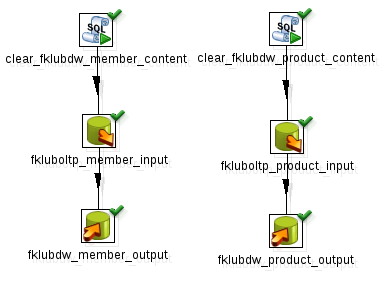
\includegraphics[width=0.5\textwidth]{img/product_memb_dim.png}
    \caption{The ETL process of creating the member and product dimension in Pentaho.}
    \label{fig:etl-process1}
\end{figure}

In \myref{fig:etl-process2} the ETL process of creating the date and time dimension and the fact table can be seen.
In the red part of \cref{fig:etl-process2} is the existing database content deleted, since Pentaho will append the new data to the old.
Then is the data extracted from the fkluboltp member table in the ``fklub\_sale\_input'' step.
After that is the date and time extracted from the ``timestamp'' field.

In the green part of \cref{fig:etl-process2} is the date part of the ``timestamp'' field sorted, duplicate rows are deleted, an id field is added and is saved to the fklubdw date dimension table. 

In the yellow part of \cref{fig:etl-process2} is the time part of the ``timestamp'' handled in the same manner as the date, and is stored in the fklubdw time dimension.

In the black part of \cref{fig:etl-process2} is the date dimension joined on the sales data, to get the corresponding date id.

In the pink part of \cref{fig:etl-process2} is the time dimension joined on the result of the black part to get the corresponding time id.
In the end is the unnecessary data removed and the fact table is saved in the fklubdw fact table. 

\begin{figure}[H]
    \centering
    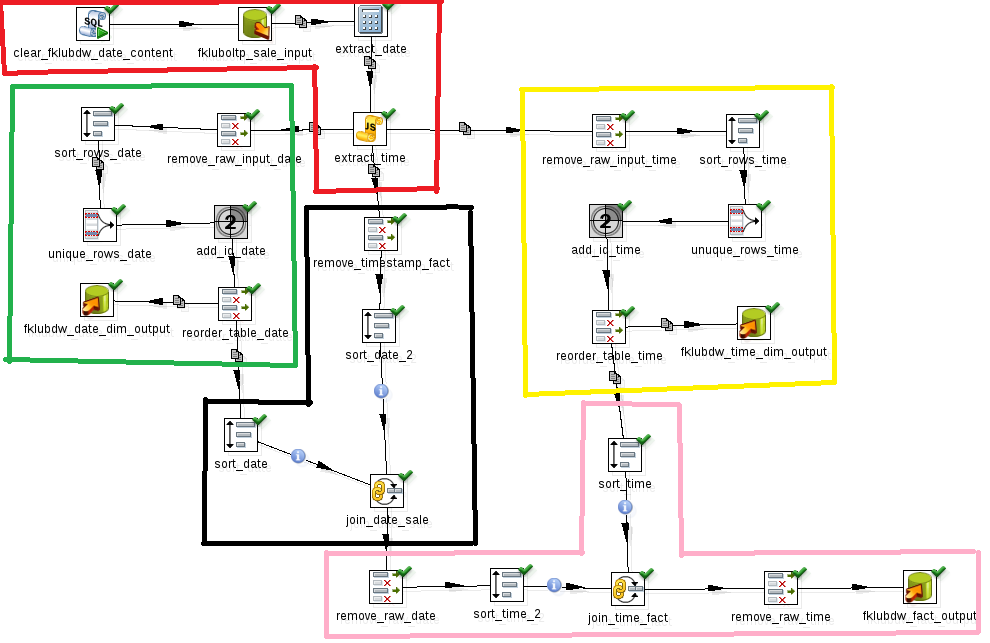
\includegraphics[width=1.0\textwidth]{img/date_time_fact.png}
    \caption{The ETL process of creating the time and date dimension and the fact table in Pentaho.}
    \label{fig:etl-process2}
\end{figure}
